\documentclass[a5j]{jsarticle}
\usepackage[dvipdfmx]{graphicx}
\graphicspath{{../graph/}}

\title{ビーム照射化における偏極陽子標的の偏極度低下の推定}

\author{東北大学理学研究科 松井貴哉}
\date{\today}
\begin{document}
\maketitle
\part{研究背景}

\part{目的}
あああaa
\part{原理}
\section{DNP}
\subsection{ペンタセン電子の偏極}
\subsection{偏極移行}
\subsection{スピン拡散}
\subsection{偏極の蓄積}
偏極度の時間発展は次式の微分方程式で表される。
$P(t)$は時刻$t$における偏極度、$P_e$はドープされた重水素化ペンタセン中の電子偏極度、$P_th$は熱平衡状態における偏極度、$T_D$は偏極生成時定数、$T_L$はDNP中の偏極緩和時定数である。
ただし、


\section{NMR}


\part{解析}

\section{微分方程式の設定}
偏極度の時間発展の様子は次のような微分方程式で記述できる。
\begin{equation}
  \frac{dP(t)}{dt}=\frac{(P_e-P(t))}{T_D}-\frac{P(t)-P_th}{T_L}
\end{equation}
P(t)は時刻tにおけるナフタレン単結晶の偏極度、$P_e$はペンタセン中の電子の偏極度、
$P_th$は熱平衡時のナフタレン単結晶の偏極度、$T_D$は偏極発展時の偏極生成時定数、 $T_L$はレーザ照射下の偏極緩和時定数を表す。


放射損の効果として以下の強度効果と積分効果を仮定した。
・強度効果:ビーム照射下の標的温度が上昇することによるスピン格子緩和時間の減少
・積分効果:ビーム照射によって結晶中のC-C,C-H結合が切断され、偏極生成、移行効率が悪化
強度効果をビーム強度に比例する項、積分効果をビーム強度、照射時間に比例する項として次式のように取り入れた。
また、ビームのon/off切り替えや強度変更の際、温度が平衡に達するのに有限の時間を要することを考慮し、強度効果には補正を行った。
この微分方程式は解析解を持たないため、数値計算を用いる。

\begin{equation}
  \frac{dP}{dt}=\frac{(P_e-P(t))}{T_D}-P(t)(\frac{1}{T_L}+\alpha I t_{beam}+\beta{1-\exp(-\frac{t_{switch}}{\gamma})})
\end{equation}
ここで、$\alpha$は積分効果の寄与の大きさを表す係数、$\beta$は強度効果の寄与の大きさを表す係数、$\gamma$は温度が平衡に達するまでの時間スケールを表す係数である。
また、ビームのon$t_{beam}$はビームの照射時間、$t_{switch}$はビーム照射のon/off切り替えや強度変更時刻からの経過時間を表す。
上式は解析的に解くことができないため、数値計算を用いてHIMAC実験で得られた偏極度推移の
データに対してフィッティングを行うことで、積分効果と強度効果の相対評価を行う。
パラメータ探索には以下の3つの手法を検討し、最も精度よくフィットできたPSO法を採用した。
\begin{enumerate}
  \item Grid Search
  \item Levenberg–Marquardt(LM)法
  \item 粒子群最適化(PSO)法(Particle Swarm Optimize)
\end{enumerate}

\section{Particle Swarm Optimize}

上記の微分方程式は6つのパラメータを持つ。
パラメータの数が多いこと、新たに設定したパラメータのオーダーから決定する必要があることから、
一般的に用いられるGrid Searchは探索に時間がかかりすぎるため不適切である。
そこで、本研究では最初に最適パラメータの検討をつけるためにParticle Swarm Optimize法を採用した。
Particle Swarm Optimize法(以下PSO法)はパラメータ探索方法の一つであり、多数のパラメータを用いた探索をGrid Searchと比較して
短時間で行うことができる。




\part{解析結果}
\begin{figure}[h]
  \centering
  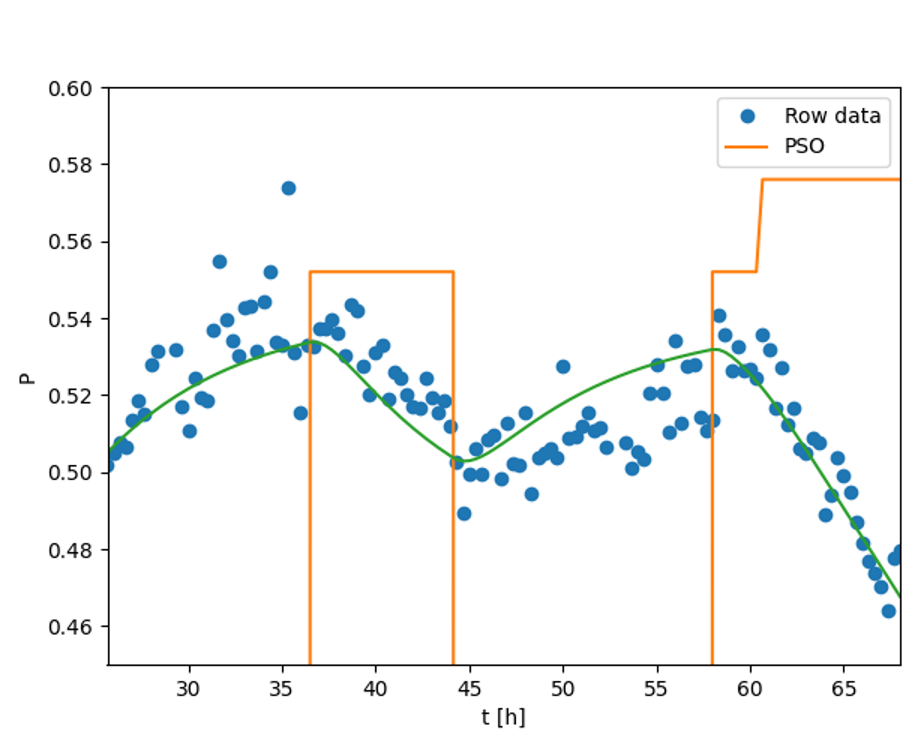
\includegraphics[width=7cm]{graph/fit.png}
  \caption{実験データ(点)と最適パラメータを用いた時のフィット結果(実線)}
\end{figure}
\section{各パラメータの数値}

\part{考察}
\section{ビーム照射中の緩和効果の比較}
\begin{figure}[h]
  \centering
  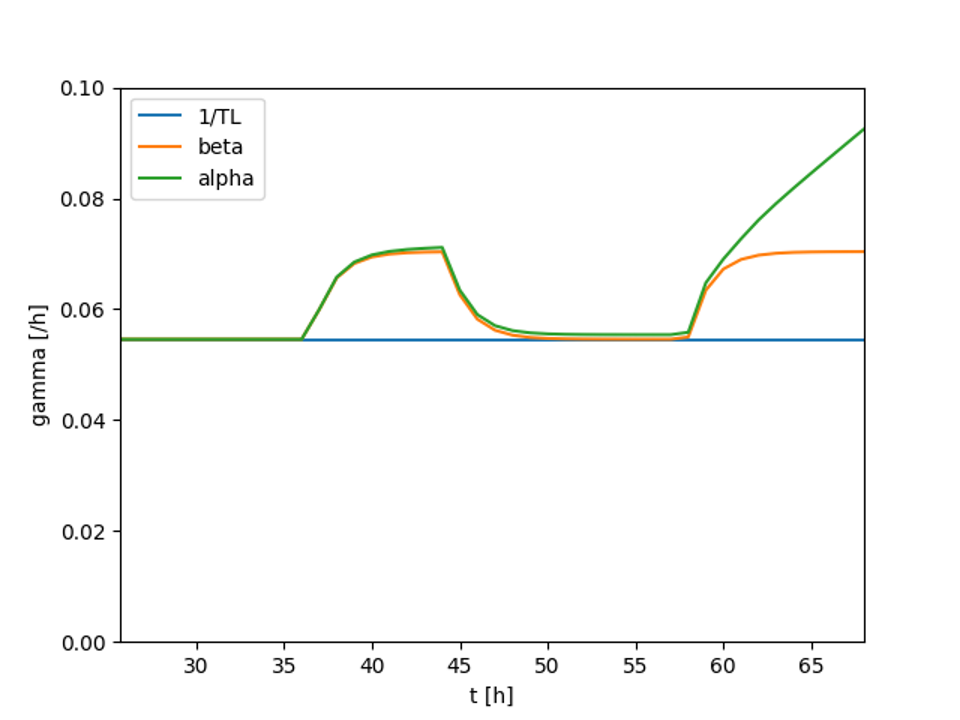
\includegraphics[width=10cm]{graph/comparison.png}
  \caption{ビーム照射中の緩和効果の比較}
\end{figure}

\section{長時間・大強度ビーム照射時の減偏極予想}
\begin{figure}[h]
  \centering
  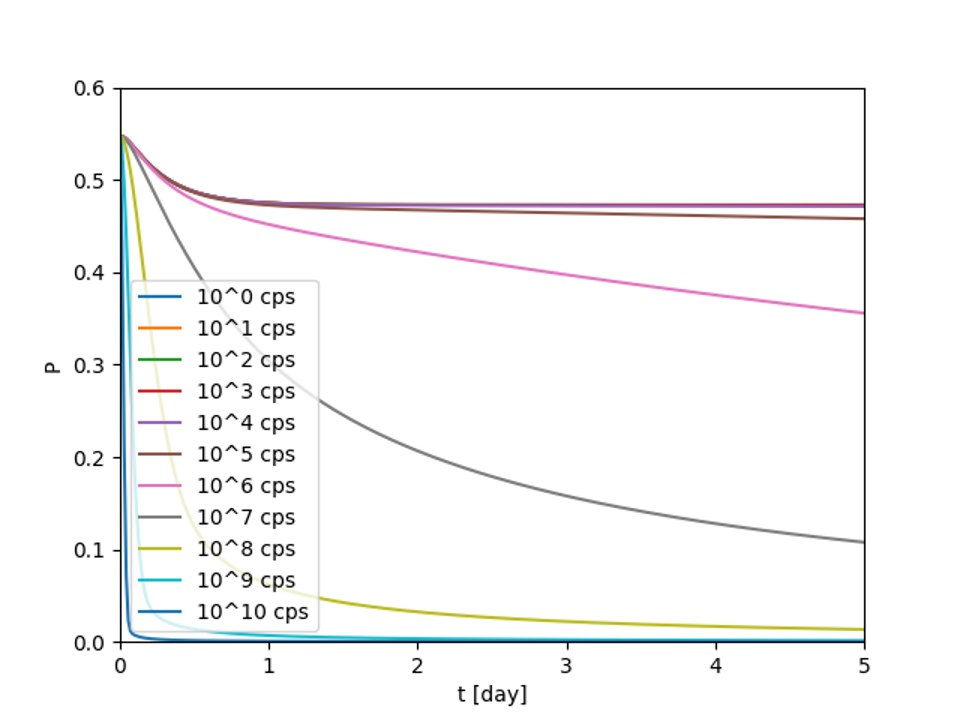
\includegraphics[width=10cm]{graph/longtime.png}
  \caption{長時間・大強度ビーム照射時の減偏極予想}
\end{figure}

\section{ビーム実験の最適ビーム強度と最適ビームタイム}
\subsection{スピン相関係数を十分な精度で測定するために必要な収量}
\subsection{収量と標的偏極度、ビーム強度、照射時間の関係}
\subsection{要求される偏極度、強度、時間}
これらの値は互いに積か商の関係になっているはずなので、全体としての必要値をもとに考える。
各値について上限と下限が存在するため、それらをもとに範囲を絞っていくことになりそう。
最終的には時間を決め打ちして強度のオーダーを決定したい。
ただ、放射損による減偏極の影響で標的偏極度が時間変化することを考慮すると単純な積では考えられないかも。

\part{今後の展望}
\section{pターフェニルの開発}
\subsection{偏極度とHIMAC実験}

\end{document}